\documentclass[main.tex]{subfiles}\begin{document}

\chapter{Implementation}
\label{chap:impl}
This chapter provides the implementation details of the outlined concept of the previous chapter.
\section{System Setup}
It is necessary to perform all experiments on the same machine to ensure a consistent comparison.
We implement all algorithms and further architecture on a Lenovo IdeaPad 5 Pro,
which runs Linux Ubuntu 20.04.5. The laptop has an AMD Ryzen 7 5800H CPU and 16 GB of RAM.

We install the most recent ROS distribution, \textit{ROS Noetic Ninjemys}\footnote{\href{http://wiki.ros.org/noetic}{http://wiki.ros.org/noetic}}, as well as 
\textit{realsense-ros}\footnote{\href{https://github.com/IntelRealSense/realsense-ros/tree/ros1-legacy}{https://github.com/IntelRealSense/realsense-ros/tree/ros1-legacy}} with all additional dependencies.
Note that the version of \textit{realsense-ros} changed over the course of this work. 
 
\section{Plane Detection Algorithms}
In Chapter~\ref{chap:Background}, we provide detailed information about the algorithms we select in Section~\ref{sec:pdaselection}.
The following subsections deal with the implementation details thereof. 
Note that the subsections of RSPD and OPS are joined due to a lack of noticeable difference in implementation details.

\subsection{RSPD \& OPS}
We implement RSPD\footnote{\href{https://github.com/abnerrjo/PlaneDetection}{https://github.com/abnerrjo/PlaneDetection}} and OPS\footnote{\href{https://github.com/victor-amblard/OrientedPointSampling}{https://github.com/victor-amblard/OrientedPointSampling}} using their respective open source implementations on GitHub.
Note that, while the implementation of RSPD is provided by one of the authors, we could not determine whether the user who uploaded his implementation of OPS is affiliated with \citeauthor{Sun_Mordohai_2019}~\cite{Sun_Mordohai_2019}.
Both methods are implemented in C++ and depend on the C++ linear algebra library \textit{Eigen}\footnote{\href{https://eigen.tuxfamily.org/index.php}{https://eigen.tuxfamily.org/index.php}},
and the C++ API of the Point-Cloud Library~\cite{Rusu_ICRA2011_PCL}, \textit{libpcl-dev}.

\subsection{3D-KHT}

The authors of 3D-KHT, provide an implementation, in form of a Visual Studio project, on their website\footnote{\href{https://www.inf.ufrgs.br/~oliveira/pubs_files/HT3D/HT3D_page.html}
    {https://www.inf.ufrgs.br/~oliveira/pubs\_files/HT3D/HT3D\_page.html}}. Since the laptop we use does not run Windows, we use \textit{cmake-converter}\footnote{\href{https://cmakeconverter.readthedocs.io/en/latest/use.html}{https://cmakeconverter.readthedocs.io/}} to convert
the solution to a CMake project we can build using \textit{make}. The dependencies of this implementation include the C++ library \textit{Dlib}~\cite{dlib09}, as well as the OpenGL Utility Toolkit 
\textit{GLUT}\footnote{\href{https://www.opengl.org/resources/libraries/glut/glut\_downloads.php}{https://www.opengl.org/resources/libraries/glut/glut\_downloads.php}}. 
Lastly, the multi-processing API OpenMP\footnote{\href{https://www.openmp.org/}{https://www.openmp.org/}} is required as well.

\subsection{OBRG}
\label{sec:impl-obrg}
To our knowledge, no open-source implementation is available for the algorithm.
We, therefore, use our own implementation, which can be found on our Github repository\footnote{\href{https://github.com/lupeterm/OBRG}{https://github.com/lupeterm/OBRG}}.

We implement the algorithm using python. We choose to write our own octree implementation for spatial subdivision of our point cloud, since
the implementation of public libraries like \textit{open3d}~\cite{Zhou2018} are limited in terms of leaf node functionality.
The subdivision is followed by calculating the saliency features using \textit{open3d}'s normal estimation function.
We follow the pseudocode as stated in \cite[Algorithm~1]{Vo_Truong-Hong_Laefer_Bertolotto_2015}. We modify the insertion into the set
of regions by adding a containment check, to avoid redundancy of regions. By reducing the number of regions (incl. redundancies), we also
reduce the total calculation time.

% It is worth noting that the choice of implementation using python is inferior considering calculation time when compared with an equivalent implementation in C++. Writing an optimized implementation in C++ would, therefore, go beyond the scope of this work, as the optimization of
% a single method is not our focus.



\section{2D-3D-S}
\label{sec:gtseg}
The \textit{2D-3D-S} dataset provides a ground truth in form of annotated point clouds corresponding to 13 object classes. Since these annotated objects are not
always planar, we cannot use them for the evaluation of plane detection algorithms. Thus, we create a ground truth that focuses on planar structures.
We use the open-source 3D point cloud and mesh processing software \textit{CloudCompare}\footnote{\href{https://www.danielgm.net/cc/}{https://www.danielgm.net/cc/}} to visualize a scene and manually segment included planes.
Because we cannot assume all walls to be planar or that, e.g., the tops or three adjacent tables always form the same number of planes (see Figure~\ref{fig:tables}), we
have to view each point cloud and segment the included planes manually. An exemplary before-and after-segmentation is shown below in Figure~\ref{fig:gtseg}.
\begin{figure} [H]
    \begin{subfigure}{0.5\textwidth}
        \centering
        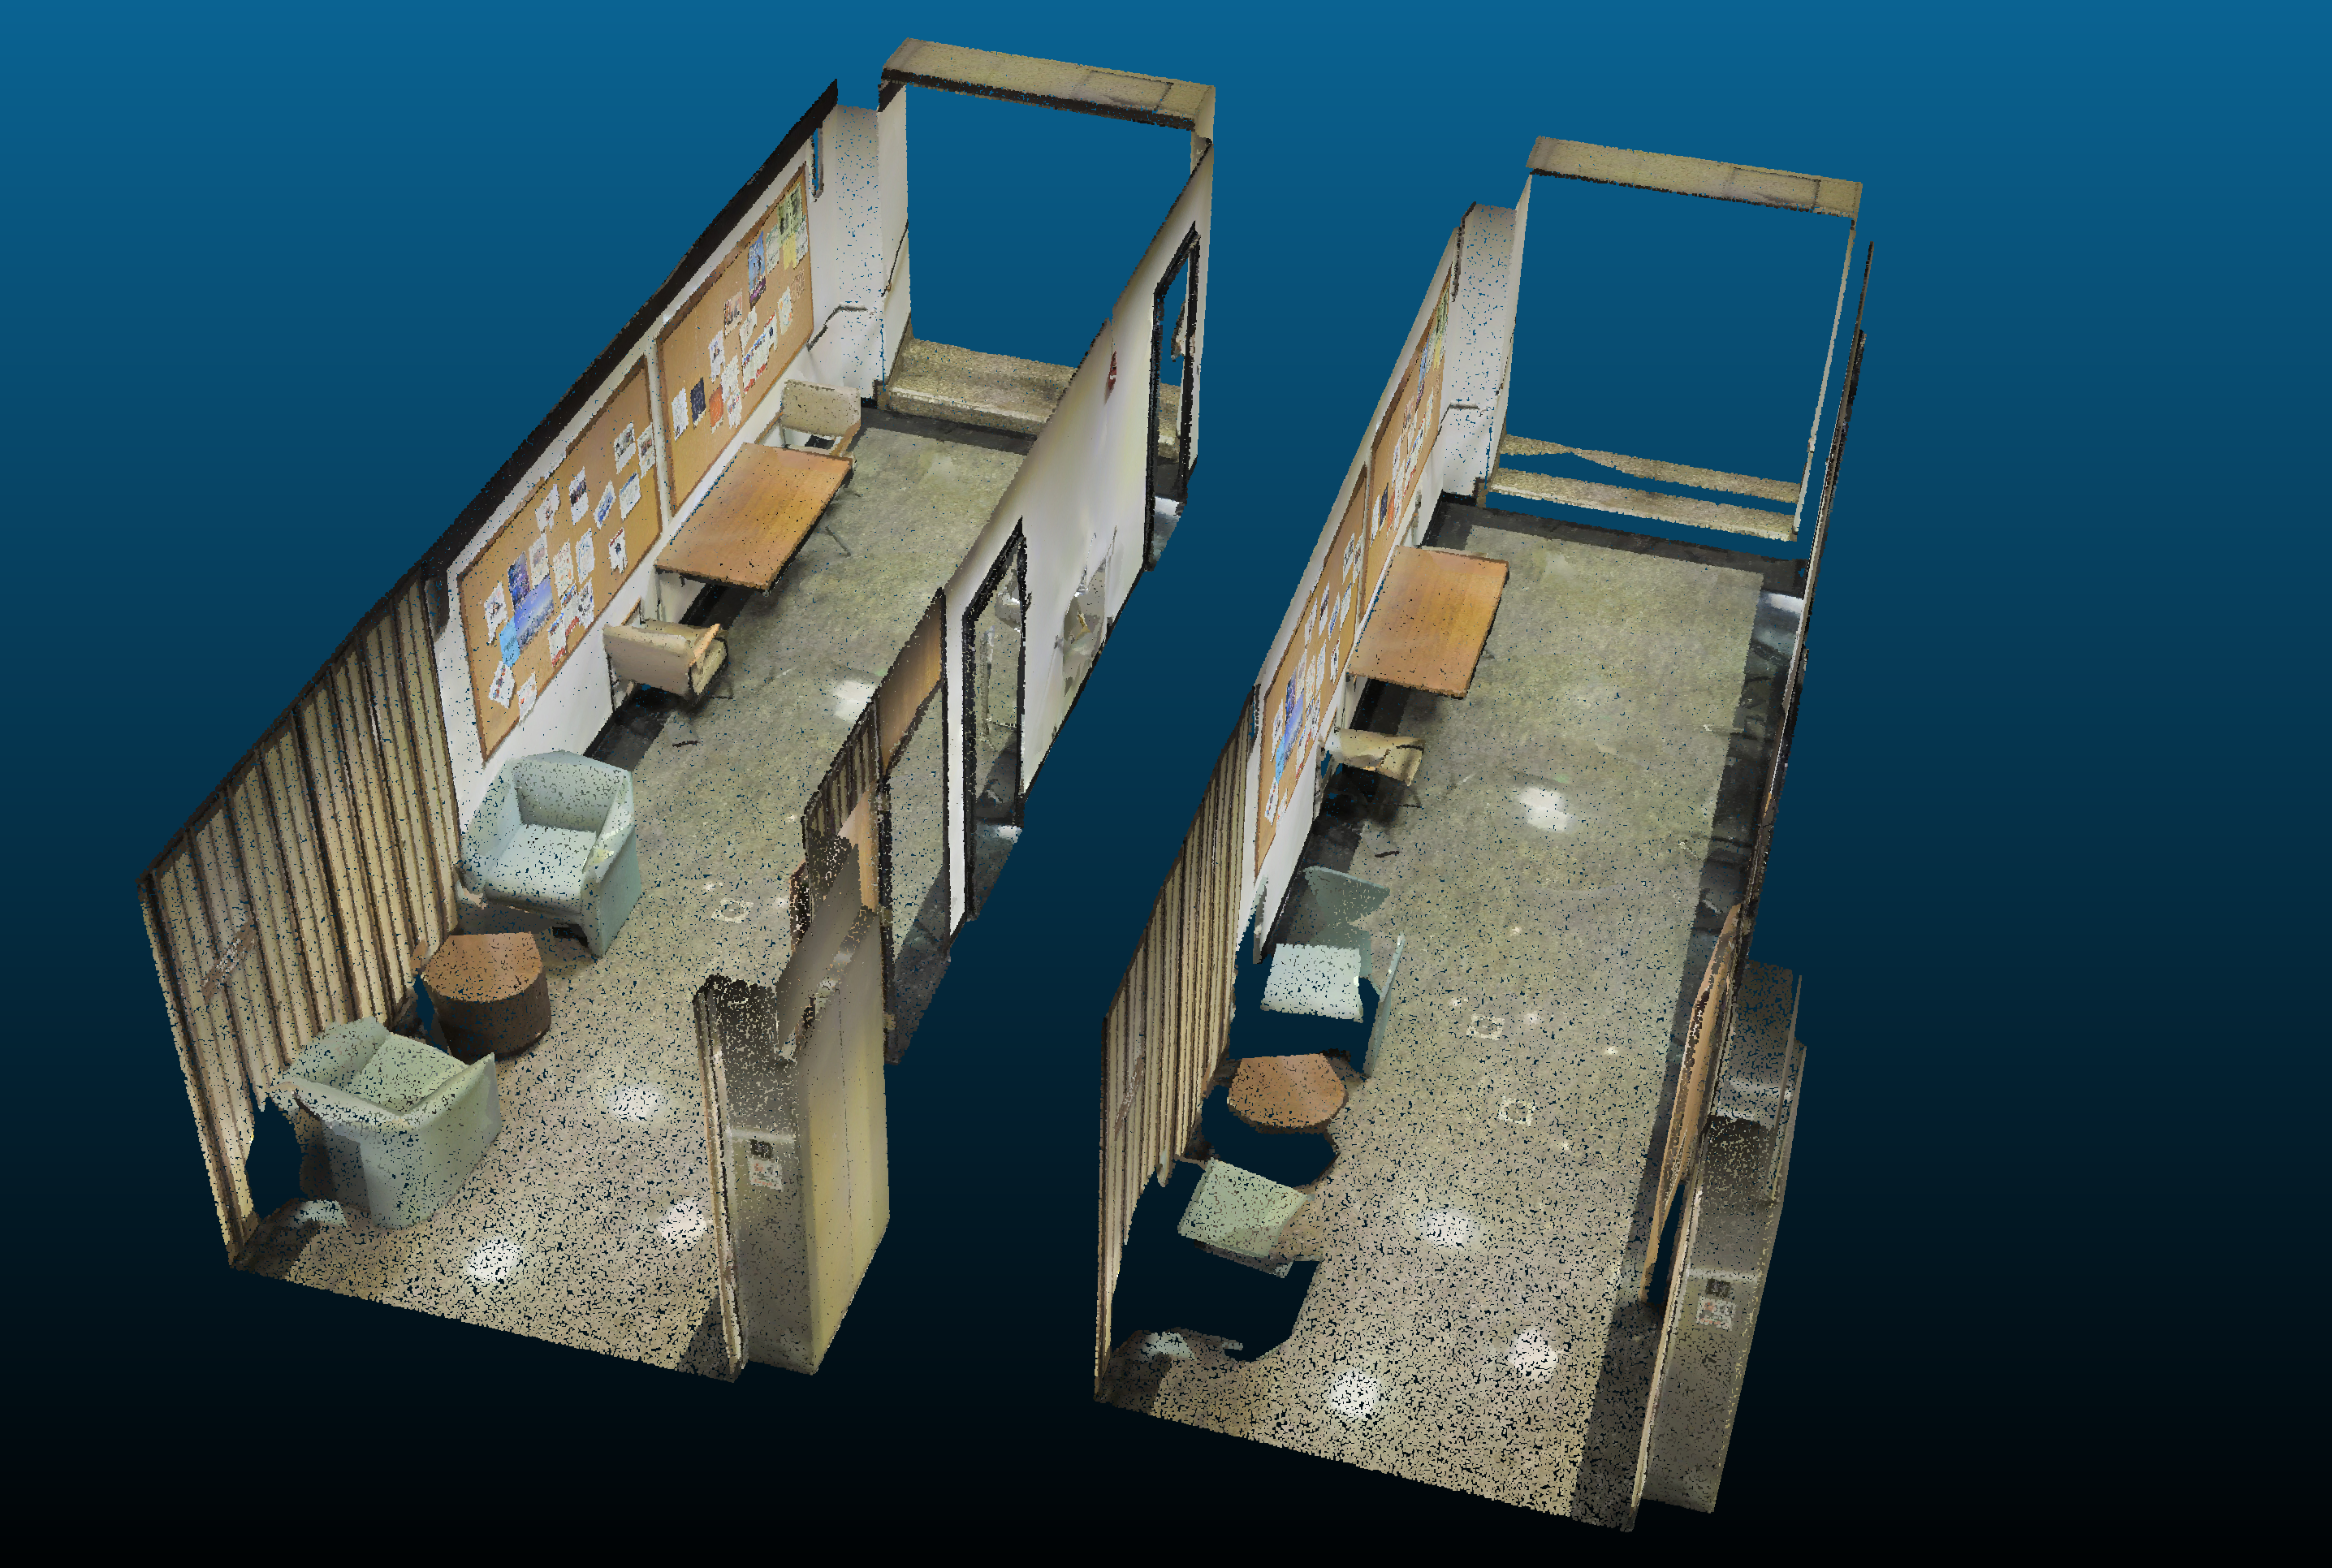
\includegraphics[width=.9\linewidth]{images/gtseg.png}
        \caption[Ground Truth Segmentation]{Ground Truth Segmentation of a hallway in CloudCompare. Shown is the input cloud on the left and segmented planes on the right.
            Both are cropped and without ceilings for visualization purposes.}
        \label{fig:gtseg}
    \end{subfigure}
    \begin{subfigure} {0.5\textwidth}
        \centering
        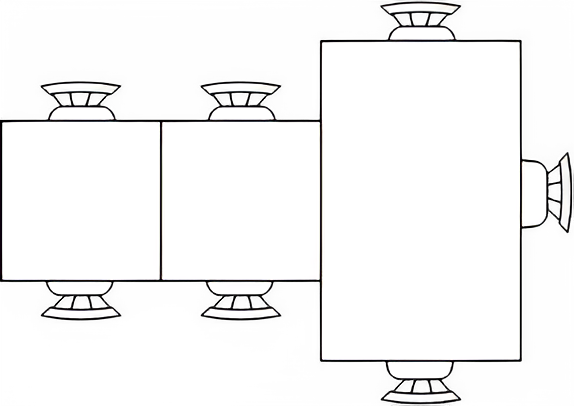
\includegraphics[width=0.9\linewidth]{images/tables.png}
        \caption[Ground Truth Table Example]{The provided ground truth considers these tables to be three separate objects. Within the context of
            plane detection, the three table tops would form exactly one plane.}
        \label{fig:tables}
    \end{subfigure}
     \caption[Ground Truth Segmentation figures]{}
\end{figure}


The manual segmentation process is very time consuming, not only because of the large amount of data but also due
to the level of subjectivity involved.
On average, the segmentation of a scene took 8-10 minutes, which, for all 272 scenes,
would result in a total of 36-45 hours. To reduce the time spent in segmentation, we perform an initial analysis of the scenes in a given area
and omit scenes that show no noticeable difference compared to others. This analysis reduces the number of segmented scenes to slightly more than half
of the total, reducing the time to 18-23 hours.

The results of the manual segmentation process are documented in Table~\ref{tab:stanfordStats}.
The table is inspired by~\cite[Table~7]{2017arXiv170201105A}. Like the original, it shows the amounts of scenes per scene type in each area.
We extended the table by adding a column dedicated to the planes included in each scene type. According to the table, a total amount of 3410 planes
are included in the dataset.


\begin{table}[H]
    \centering
    \resizebox{\textwidth}{!}{%
        \begin{tabular}{c|c|c|c|c|c|c|c||c}
            Scene Categories & Area\_1 & Area\_2 & Area\_3 & Area\_4 & Area\_5 & Area\_6 & TOTAL            & Planes \\ \hline
            auditorium       & -       & 2/2     & -       & -       & -       & -       & 2/2              & 70             \\ \hline
            conference room  & 2/2     & 1/1     & 1 /1    & 3/3     & 3/3     & 1/1     & 11/11            & 375            \\ \hline
            copy room        & 1/1     & -       & -       & -       & -       & 1/1     & 2/2              & 45             \\ \hline
            hallway          & 8/8     & 12/12   & 6/6     & 14/14   & 1/15    & 6/6     & 48/61            & 977            \\ \hline
            lobby            & -       & -       & -       & 2 /2    & 1/1     & -       & 3/3              & 207            \\ \hline
            lounge           & -       & -       & 2/2     & -       & -       & 1/1     & 3/3              & 101            \\ \hline
            office           & 16/31   & 5/14    & 10/10   & 9/22    & 4/42    & 3/37    & 48/156           & 1116           \\ \hline
            open space       & -       & -       & -       & -       & -       & 1 /1    & 1/1              & 10             \\ \hline
            pantry           & 1/1     & -       & -       & -       & /1      & 1/1     & 3/3              & 73             \\ \hline
            storage          & -       & 9/9     & 2 /2    & 4/4     & 4/4     & -       & 19/19            & 222            \\ \hline
            WC               & 1/1     & 2/2     & 2/2     & 4/4     & 4/2     & -       & 11/11            & 214            \\ \hline
                             &         &         &         &         &         &         & \textbf{139/272} & \textbf{3410}
        \end{tabular}
    }
    \caption[2S-3D-S Statistics]{2D-3D-S dataset statistics. Shown are the number of scenes per category and for how many we created a ground truth ($\#GT/\#Total$).
        Note that the rightmost column reports the number of segmented planes per scene category and does \textit{not} 
        correspond to other columns in this table.  }
    \label{tab:stanfordStats}
\end{table}


\section{FIN Dataset}
\label{sec:finimpl}
Reiterating Section~\ref{sec:datasets}, we select four scene types of the \textit{2D-3D-S} dataset for the recording of the self-created FIN
dataset. Namely, these scene types are \textit{auditorium, conference room, hallway,} and \textit{office}.
All scenes are recorded inside the \textit{Faculty of INformatik} (FIN) at Otto-von-Guericke-University in Magdeburg.
Running \textit{realsense-ros} and holding our cameras, we walk through the corresponding parts of the building while scanning to the best of our ability.
We save each incremental map update to a file for further usage.

Given the differences in spatial dimension, the recordings of each scene also differ in length and size.
The auditorium scene has a total of 296 individual time frames, the conference room scene has 113, the hallway has a total of 174, 
and the office has 125 time frames.
The FIN dataset, thereby, has a total of 708 time frames.

Since no ground truth exists for a novel dataset like this, we create a set of ground truth planes $gt_{end}$ for only the most recent update of each scene, e.g., for the entire recording.
By creating a ground truth for only the last frame of each scene, we substantially reduce the time invested in this task.
To prepare for the evaluation of a point cloud $m_t$ at a given time $t$, we crop all planes in $gt_{end}$ by removing all points that are not present in $m_t$.
Figure~\ref{fig:dynGT} shows the final point cloud and the manually created ground truth $gt_{end}$ of the \textit{hallway} scene on the far right. 
On the left thereof, two point clouds of earlier stages of the recording are shown, as well as their dynamically created ground truth. 
We speed up this expensive process by employing a KD-Tree neighbor search with a small search radius since we only need to know whether a certain point is present or not.

\begin{figure}[H]
    \centering
    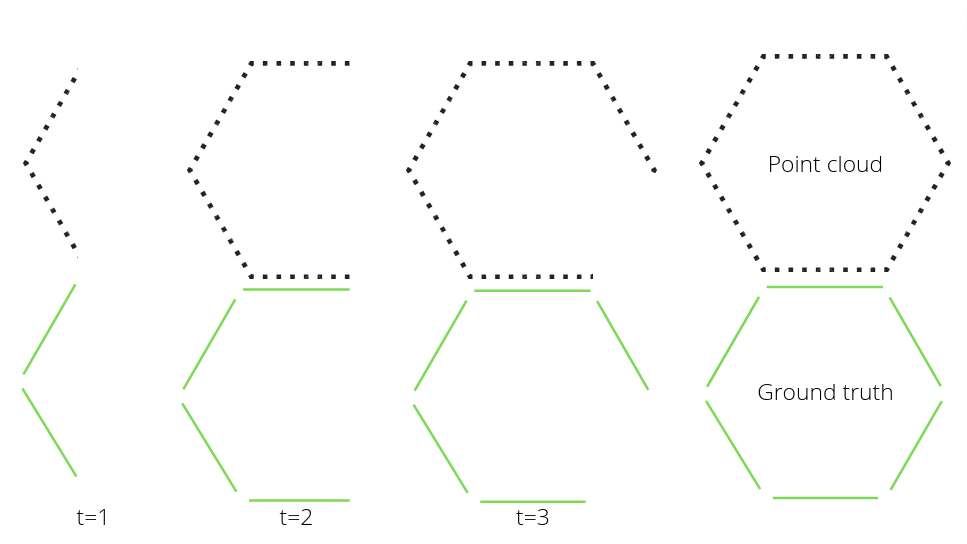
\includegraphics[width=15 cm]{images/dynamic_eval.png}
    \caption[Dynamic Ground Truth Generation]{Dynamic ground truth generation shown by the example of three point clouds from the
    \textit{hallway} scene, as well as the corresponding ground truth. The rightmost pair shows the 
    final state of the point cloud and its ground truth.}

    \label{fig:dynGT}
\end{figure}

\end{document}
